\documentclass[tikz,border=10pt]{standalone}
\usepackage{amsmath}
\begin{document}
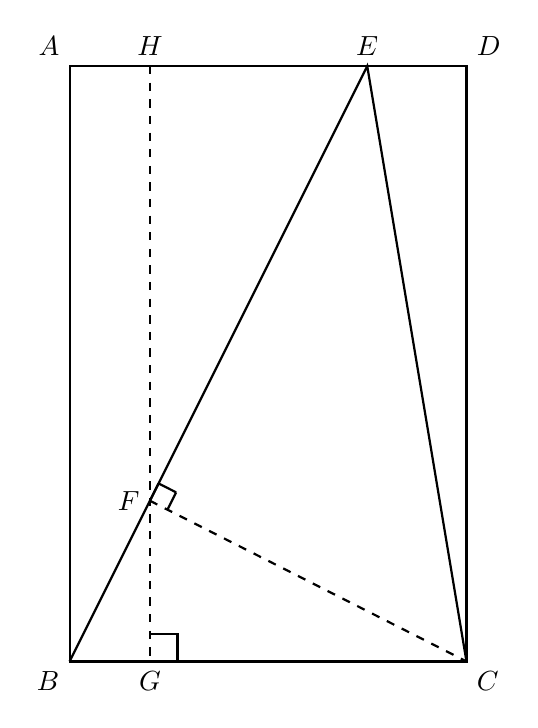
\begin{tikzpicture}[scale=1, line width=0.8pt]
  % Points
  \coordinate (A) at (0,7.56);
  \coordinate (D) at (5.04,7.56);
  \coordinate (B) at (0,0);
  \coordinate (C) at (5.04,0);
  \coordinate (E) at (3.78,7.56);
  \coordinate (H) at (1.02,7.56);
  \coordinate (G) at (1.02,0);
  \coordinate (F) at (1.02,2.04);

  % Rectangle ABCD
  \draw (A) -- (D) -- (C) -- (B) -- cycle;

  % Solid triangle BEC
  \draw (B) -- (E) -- (C);

  % Dashed lines
  \draw[dashed] (H) -- (G);
  \draw[dashed] (F) -- (C);

  % Right-angle marks
  \draw (1.02,0.35) -- (1.37,0.35) -- (1.37,0);
  \draw (1.243,1.927) -- (1.353,2.147);
  \draw (1.353,2.147) -- (1.13,2.26);
  \draw (1.13,2.26) -- (1.02,2.04);

  % Labels
  \node[above left] at (A) {$A$};
  \node[above right] at (D) {$D$};
  \node[below left] at (B) {$B$};
  \node[below right] at (C) {$C$};
  \node[above] at (E) {$E$};
  \node[above] at (H) {$H$};
  \node[below] at (G) {$G$};
  \node[left] at (F) {$F$};
\end{tikzpicture}
\end{document}
